\documentclass[]{article}
\usepackage{caption,subcaption,graphicx,float,url,amsmath,amssymb,tocloft}
\usepackage[hidelinks]{hyperref}
\usepackage[toc,acronym,nonumberlist]{glossaries}
\setacronymstyle{long-short}
\usepackage{glossaries-extra}
\graphicspath{{figs/}} 
\setlength{\cftsubsecindent}{0em}
\setlength{\cftsecnumwidth}{3em}
\setlength{\cftsubsecnumwidth}{3em}

%opening
\title{
	Notes from Origins of Life\\
	Week 6: Astrobiology \& General Theories of Life
}
\author{Simon Crase}

\makeglossaries
\renewcommand{\thesection}{6.\arabic{section}}

\loadglsentries{glossary-entries}

\renewcommand{\glstextformat}[1]{\textbf{\em #1}}

\begin{document}

\maketitle

\begin{abstract}
   These are my notes from the $6^{th}$ Week of the Santa Fe Institute Origins of Life Course\cite{sfi2019}. The course aims to push the field of Origins of Life research forward by bringing new and synthetic thinking to the question of how life emerged from an abiotic world.\\
   The content and images contained herein are the intellectual property of the Santa Fe Institute, with the exception of any errors in transcription, which are my own.
   These notes are distributed in the hope that they will be useful,
   but without any warranty, and without even the implied warranty of
   merchantability or fitness for a particular purpose. All feedback is welcome,
   but I don't necessarily undertake to do anything with it.

\end{abstract}

\setcounter{tocdepth}{2}
\tableofcontents

\listoffigures

\section{Introduction}

Lecturer: Chris Kempes

Ultimate goal is to provide a general theory of Life, one capable of uncovering the history we know about, but also bounding the possibilities for other types of life, and helping us recognize other forms of life. In this unit we'll discuss the search for life beyond Earth and how origins of life fits into this effort. We'll also discuss general evolutionary processes and abstract life. 

\section{Origins of Life and Astrobiology}

Lecturer: Sara Imari Walker

Why is Origins so important to Astrobiology? We want to be able to identify living organisms on another planet. We can send robotic missions within the Solar System, but we have only a small amount of data for exoplanets.

 What makes worlds with life different--Figure \ref{fig:Jupiter:Tellus}? Jupiter and Earth both have non-equilibrium surface features, so that isn't sufficient.

\begin{figure}[H]
	\caption{What makes worlds with life different?}\label{fig:Jupiter:Tellus}
	\begin{subfigure}[b]{0.45\textwidth}
		\caption{Jupiter}\label{fig:Jupiter}
		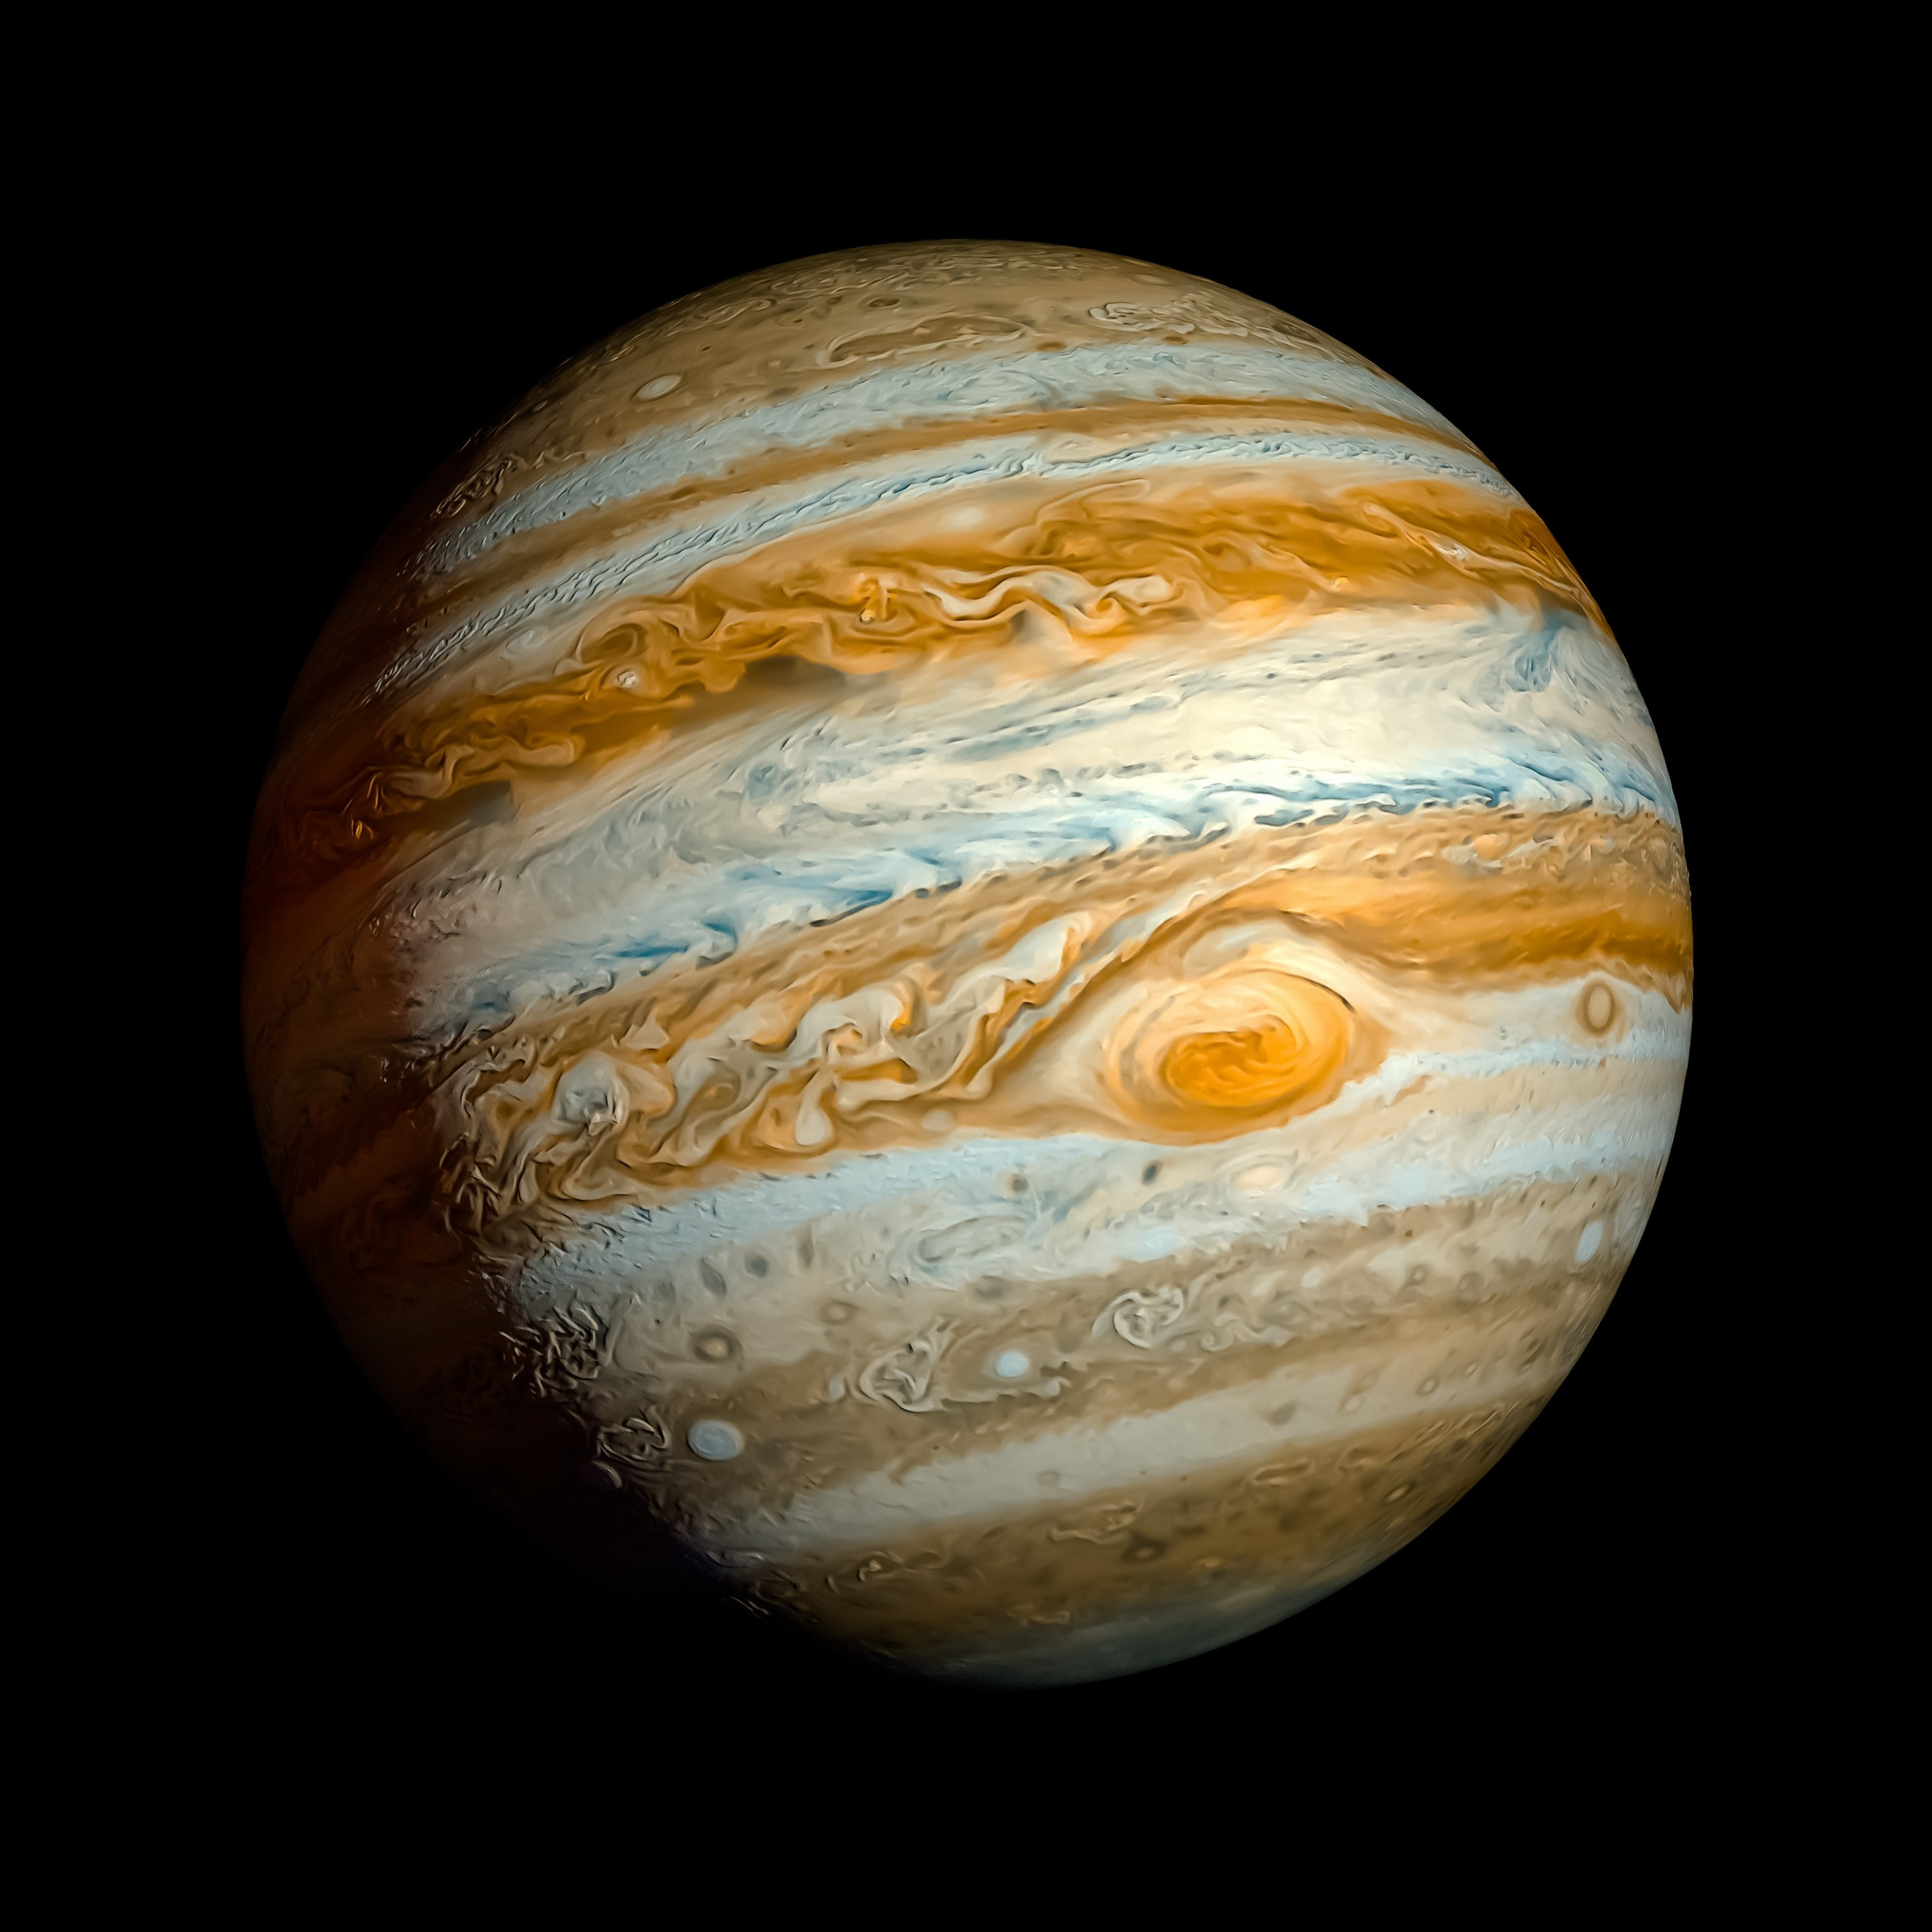
\includegraphics[width=\textwidth]{Jupiter}
	\end{subfigure}
	\begin{subfigure}[b]{0.45\textwidth}
		\caption{Earth at night}\label{fig:Earth}
		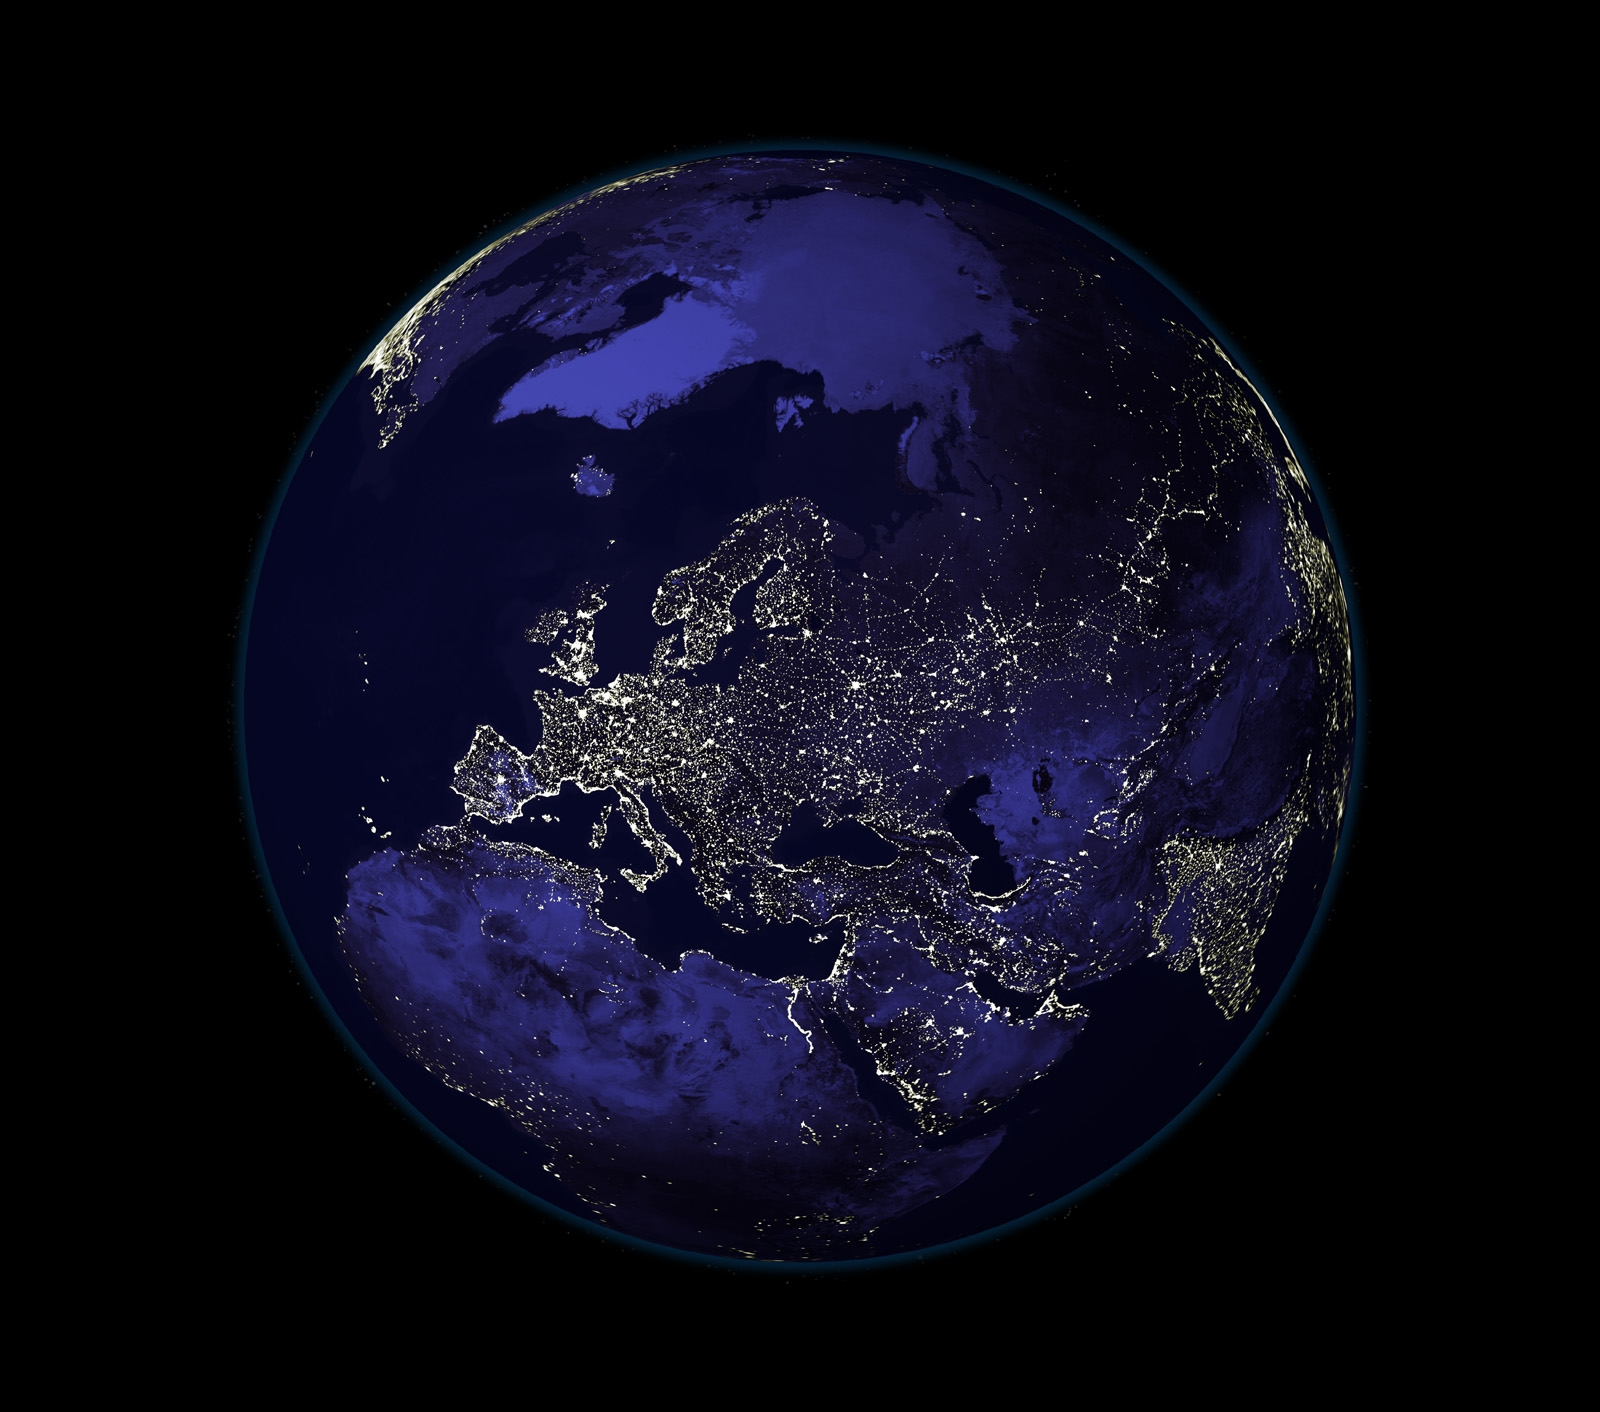
\includegraphics[width=\textwidth]{Tellus}
	\end{subfigure}
\end{figure}

Figure \ref{fig:P:Life} shows how we can constrain the probability of Life.  Our Theory should be able to explain the differences in Figure \ref{fig:Jupiter:Tellus}.

\begin{figure}[H]
	\caption{Rate of abiogenesis in a prebiotic environment as a function of its physical and chemical conditions}\label{fig:P:Life}
	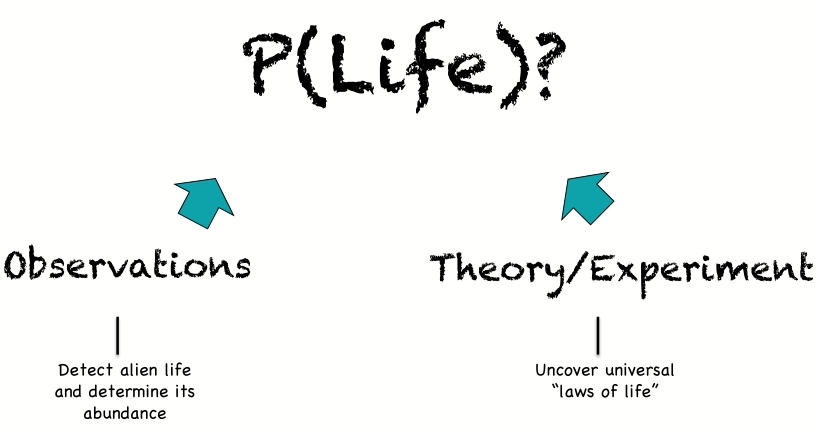
\includegraphics[width=0.9\textwidth]{P_Life}
\end{figure}

''Base metals can be transmuted into gold by stars, and by intelligent beings who understand the processes that power stars, and by nothing else in the universe''--David Deutsch\cite{deutsch2011beginning}.

We want a theory that allows us to understand the diversity of Figure \ref{fig:Earth}.

\section{Exoplanets}

\subsection{The Habitable Zone}

Lecturer: Elizabeth Tasker

Figure \ref{fig:exoplants} shows the number of exoplanets known by discovery technique.\cite{nasa2019Explonet}.

\begin{figure}[H]
	\caption{Exoplanets by discovery technique}\label{fig:exoplants}
	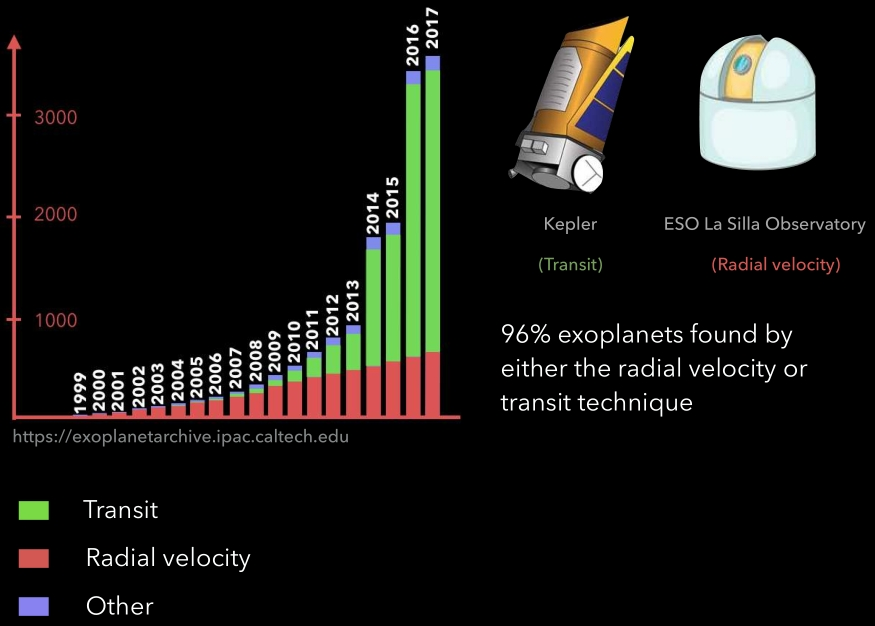
\includegraphics[width=0.9\textwidth]{Exoplanets}
\end{figure}

There are two main techniques:
\begin{itemize}
	\item Radial velocity or Doppler wobble:Orbit with planet causes the
	star to wobble, creating a
	periodic shift in wavelength
	\item Transit: Dip in light as planet crosses
	our line of sight to the star
\end{itemize}

Typically this tells us up to two things about the planet, none of which measurable properties directly relates to surface conditions:
\begin{itemize}
	\item Radius of planet
	\item Mass of planet
\end{itemize}

Our next generation of instruments
aim at atmospheric composition

Rank by most interesting target for habitability

\begin{itemize}
	\item Easiest to recognise Earth-like life 	(water \& carbon-based chemistry)
	\item Needs to be detectable 	(surface water needed)
	\item How much insolation does an 	Earth-like planet need?
\end{itemize}

\begin{figure}[H]
	\caption{Classical Habitable Zone}\label{fig:classical:habitable:zone}
	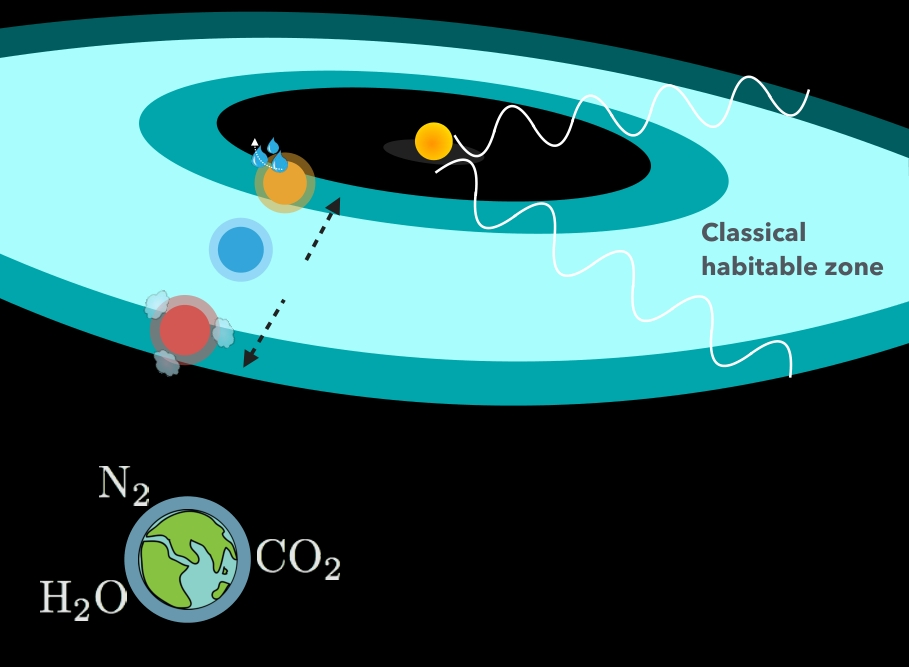
\includegraphics[width=0.9\textwidth]{ClassicalHabitableZone}
\end{figure}

Figure \ref{fig:optimistic:habitable:zone} depicts the Optimistic Habitable Zone, based on empirical data that Venus \& Mars once had surface liquid water 1 - 3.8 Gyrs ago \cite{kasting1993habitable}.
\cite{kopparapu2013habitable}
\begin{figure}[H]
	\caption{Optimistic Habitable Zone }\label{fig:optimistic:habitable:zone}
	    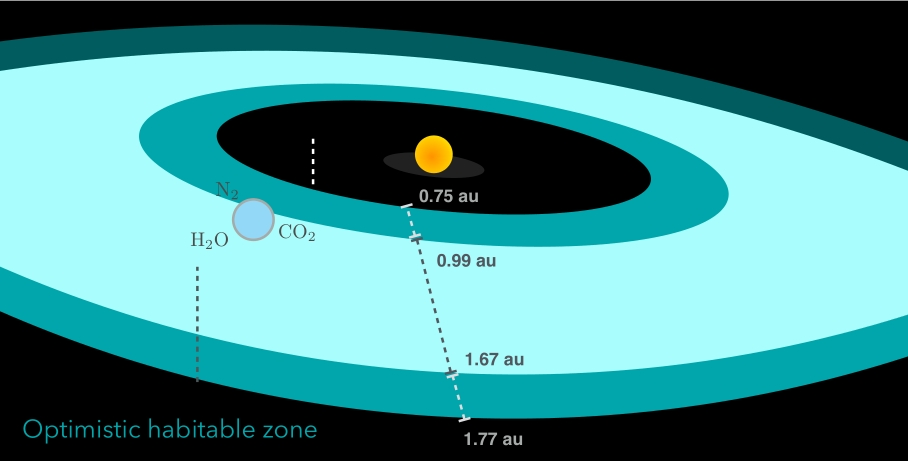
\includegraphics[width=0.9\textwidth]{OptimisticHabitableZone.jpg}
\end{figure}

The classical habitable zone is only for an Earth-like planet. Different planets might have a habitable zone at a different location, or not at all.

Are the exoplanets in Figure \ref{fig:are:these:earthlike} Earth-like? We don’t know. Can only say: If we found another habitable Earth-like planet, it would be in the habitable zone.

\begin{figure}
	\caption{Are these exoplanets Earth-like?}\label{fig:are:these:earthlike}
	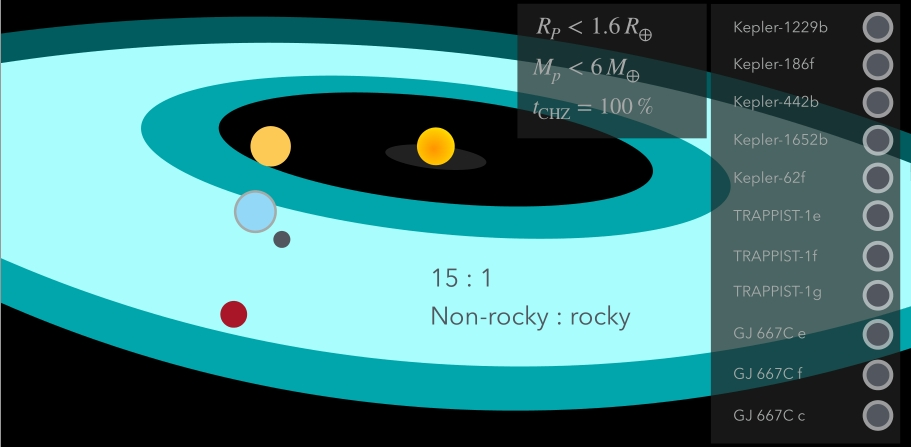
\includegraphics[width=0.9\textwidth]{AreTheseEarthlike}
\end{figure}

Conclusions

\begin{itemize}
	\item We’ve discovered thousands of exoplanets, many of which are similar in
	size to the Earth.
	\item But at the moment, we have no way of knowing what their surfaces are
	like (note that the Earth and Venus are both “Earth-sized planets”.)
	\item Our next generation of telescopes will be able to detect the atmosphere
	of these worlds and tell us something about their surfaces for the first
	time.
	\item The habitable zone is a useful concept for selecting planets for the 	new telescopes, but it offers no guarantee that a planet is habitable.
\end{itemize}

See also \cite{fujii2018exoplanet} and \cite{villanueva2015unique}.

\subsection{Exoplanet Atmospheric Characterization}

Lecturer: Yuka Fujii

Exoplanet Discovery usually come with Size (mass and/or radius) and Orbit--Figure \ref{fig:discovered:exoplanets}.

\begin{figure}[H]
	\caption{Discovered Exoplanets}\label{fig:discovered:exoplanets}
	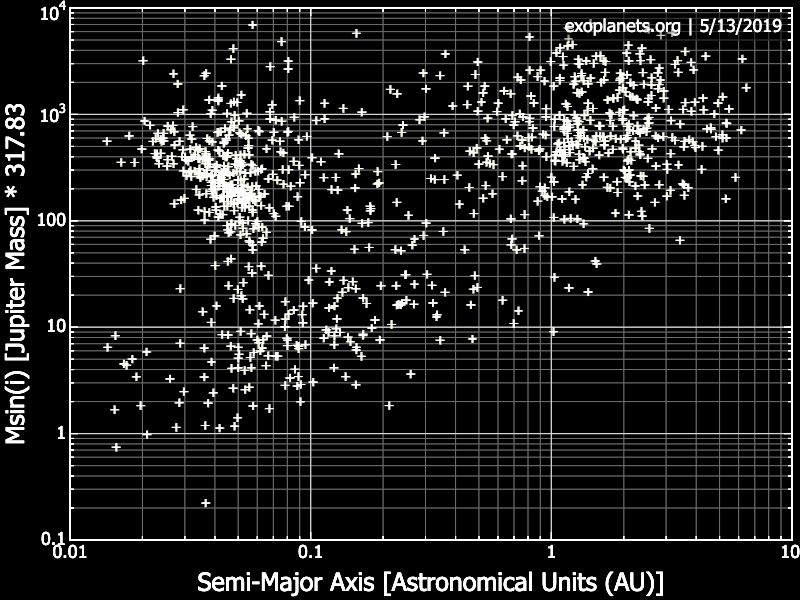
\includegraphics[width=0.9\textwidth]{ExoplanetCharacteristics}
\end{figure} 

Figure \ref{fig:spectrum:earth:twin} depicts the spectrum that we'd expect from a twin planet for Earth. At shorter wavelengths the planet scatters light--Figure \ref{fig:spectrum:earth:twin1}--and the spectrum depends on the composition of the surface; at longer wavelengths it emits infrared--Figure \ref{fig:spectrum:earth:twin2}-- and the spectrum depends on the temperature structure. Figure \ref{fig:spectrum:earth:twin3} depicts the effect of absorption by atmospheric species. For an Earth twin we'd expect to find biologically important molecules. We can scan the plant's surface as it rotates.

\begin{figure}[H]
	\caption{Spectrum of an earth twin}
	\begin{subfigure}[b]{0.45\textwidth}
		\caption{Spectrum of an earth twin}\label{fig:spectrum:earth:twin}
		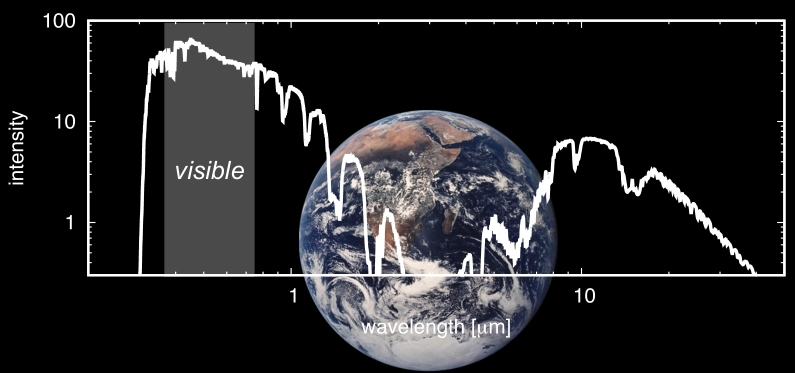
\includegraphics[width=\textwidth]{SpectrumEarthTwin}
	\end{subfigure}
	\begin{subfigure}[b]{0.45\textwidth}
		\caption{At shorter wavelengths the planet scatters light}\label{fig:spectrum:earth:twin1}
		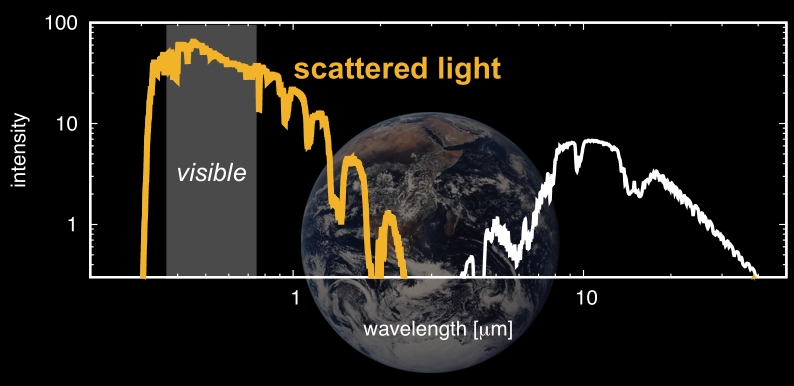
\includegraphics[width=\textwidth]{SpectrumEarthTwin1}
	\end{subfigure}
	\begin{subfigure}[b]{0.45\textwidth}
		\caption{At longer wavelengths it emits infrared}\label{fig:spectrum:earth:twin2}
		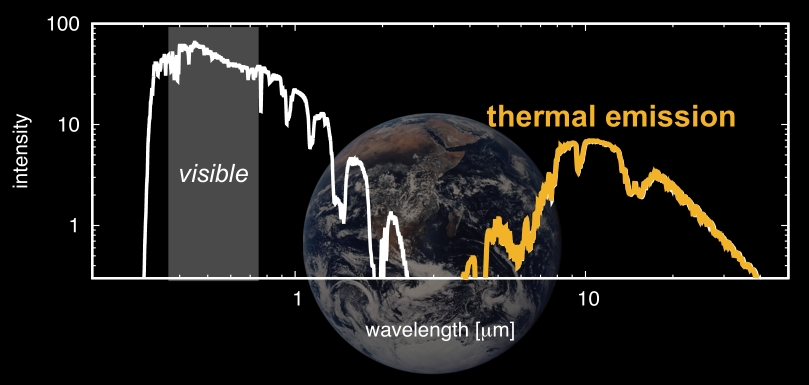
\includegraphics[width=\textwidth]{SpectrumEarthTwin2}
	\end{subfigure}
	\begin{subfigure}[b]{0.45\textwidth}
		\caption{Absorption by atmospheric species}\label{fig:spectrum:earth:twin3}
		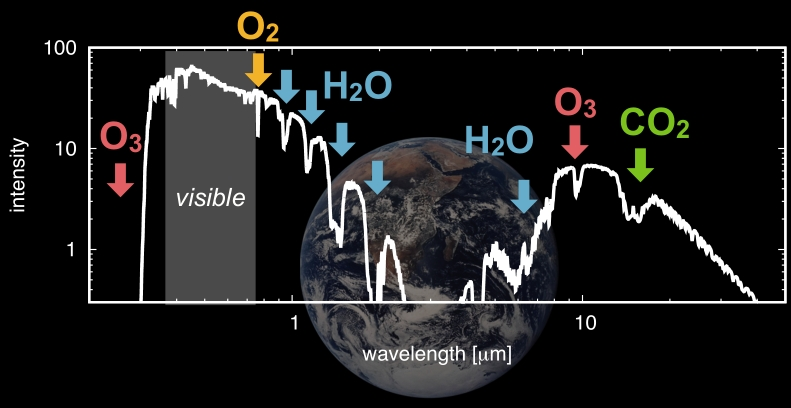
\includegraphics[width=\textwidth]{SpectrumEarthTwin3}
	\end{subfigure}
\end{figure}

Of course it is difficult to disentangle the light of the planet from the star--Figure \ref{fig:StarIsMuchBrighter}. We need to subtract the light of the star.

\begin{figure}[H]
	\caption{Unfortunately the star is many orders of magnitude brighter than its planets}\label{fig:StarIsMuchBrighter}
	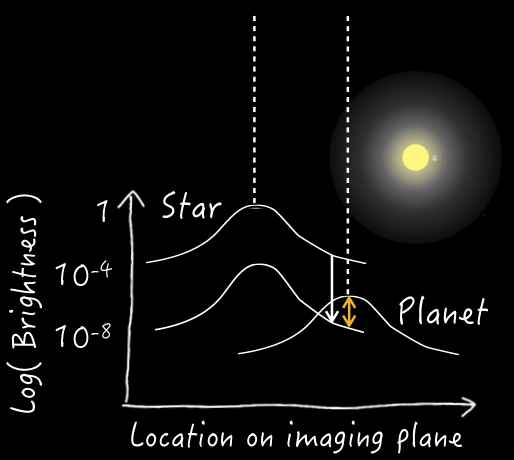
\includegraphics[width=\textwidth]{StarIsMuchBrighter}
\end{figure}

In the past decade, Direct Imaging has been successful with young hot Jupiters in wide orbits--Figure \ref{fig:young:jupiter}. See  Figures  \ref{fig:young:jupiter1}\cite{marois2010images} and Figure \ref{fig:young:jupiter2}
\cite{greenbaum2018gpi}. These planets, however, are an order of magnitude brighter than earthlike planets.

\begin{figure}[H]
	\caption{Success with Young Jupiter-like Planets in Distant Orbits}\label{fig:young:jupiter}
	\begin{subfigure}[b]{0.45\textwidth}
		\caption{}\label{fig:young:jupiter1}
		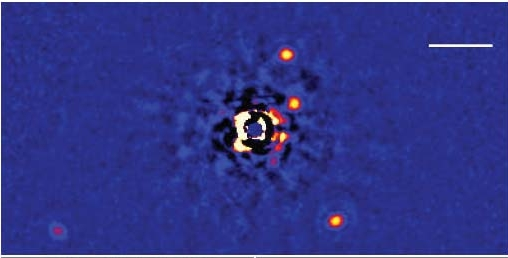
\includegraphics[width=\textwidth]{DirectImaging1.jpg}
	\end{subfigure}
	\begin{subfigure}[b]{0.45\textwidth}
		\caption{}\label{fig:young:jupiter2}
		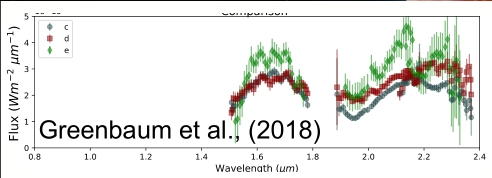
\includegraphics[width=\textwidth]{DirectImaging2.jpg}
	\end{subfigure}
\end{figure}

The discovery of transiting planets has opened up new prospects for studying exoplanet spectra--Figure \ref{fig:transiting:planets} without special instruments. A transiting planet is one that passes in front of the Star because its orbital plane is aligned with the telescope--Figure \ref{fig:transiting:planets2}. A small portion of the light is filtered through the planetary atmosphere--Figure \ref{fig:transiting:planets3}.
\begin{figure}[H]
	\caption{Transiting Planets}\label{fig:transiting:planets}
	\begin{subfigure}[t]{0.3\textwidth}
		\caption{}\label{fig:transiting:planets1}
		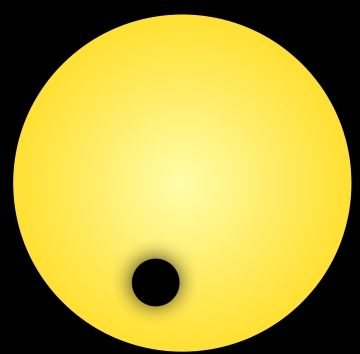
\includegraphics[width=\textwidth]{TransitingPlanets1}
	\end{subfigure}
	\begin{subfigure}[t]{0.3\textwidth}
		\caption{Passing in front}\label{fig:transiting:planets2}
		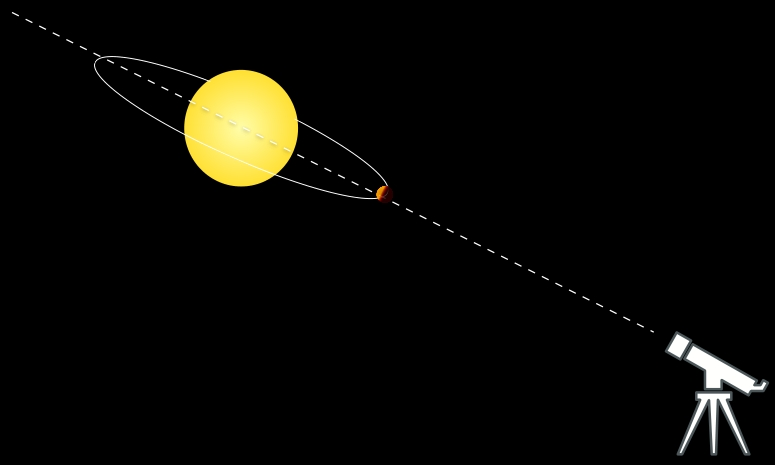
\includegraphics[width=\textwidth]{TransitingPlanets2}
	\end{subfigure}
	\begin{subfigure}[t]{0.3\textwidth}
		\caption{Transmission Spectroscopy}\label{fig:transiting:planets3}
		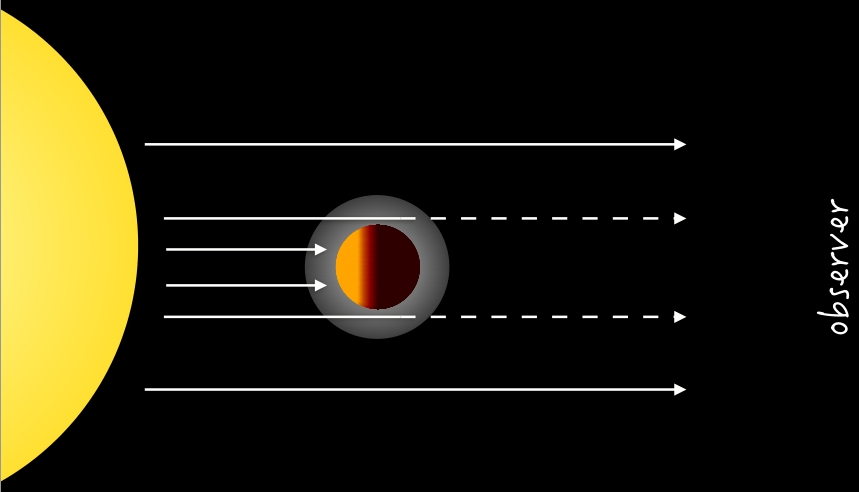
\includegraphics[width=\textwidth]{TransitingPlanets3}
	\end{subfigure}
\end{figure}
	

Summary: Key observations to characterize atmospheres (and surfaces) of exoplanets
\begin{itemize}
	\item Direct Imaging
	\item  Transmission spectroscopy
	\item  Secondary eclipse
	\item  Phase curves
\end{itemize}
Using these techniques, how would you find life on an Earth-twin?

\cite{sagan1993search}
\cite{kaltenegger2017characterize}
\cite{fujii2018exoplanet}

\cite{robinson2011earth}

\cite{deming2013infrared}
\cite{knutson2007map}

\section{What is Life?}

\subsection{Constraining the Definition of Life}

''... living matter, while not eluding the laws of physics as established up to date, is likely to involve other laws of physics hitherto unknown''\cite{schrodinger1944life}

\begin{figure}[H]
	\caption{History of Unifications in Physics}
	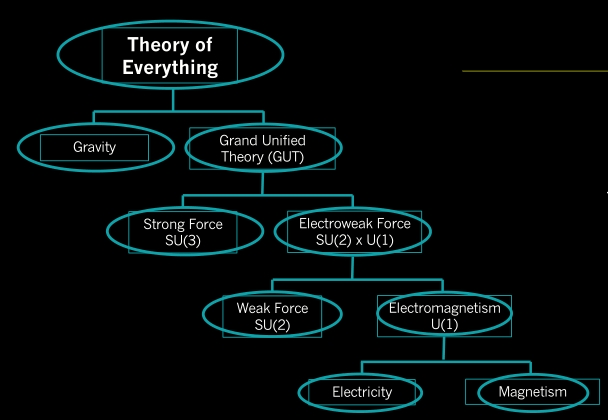
\includegraphics[width=0.9\textwidth]{Unifications}
\end{figure}
''The theory of everything is a theory of everything except of those things that theorize''--David Krakauer.

Examples of "Life"
\begin{itemize}
	\item The Cell as a unit of Life--Figure \ref{fig:cell}
	\item Metabolism--Figure \ref{fig:metabolism}
	\item Tardigrade--an extremophile that can live in space--Figure \ref{fig:tardigrade}. Maybe we should think about the widest set of confitions under which life \textit{can} exist.
	\item Two-headed planarian worms--Figure \ref{fig:2headed:planaria}. What is the limit for viable life?\cite{levin2019planarian}
	\item What is we replace RNA/DNA with XNA?
	\item Social Insects--Figure \ref{fig:social:insects}. Is the super-organism "alive"?\cite{pratt2015psychology}
	\item City--Figure \ref{fig:city}
\end{itemize}

\begin{figure}[H]
	\caption{The Cell as a unit of Life}\label{fig:cell}
	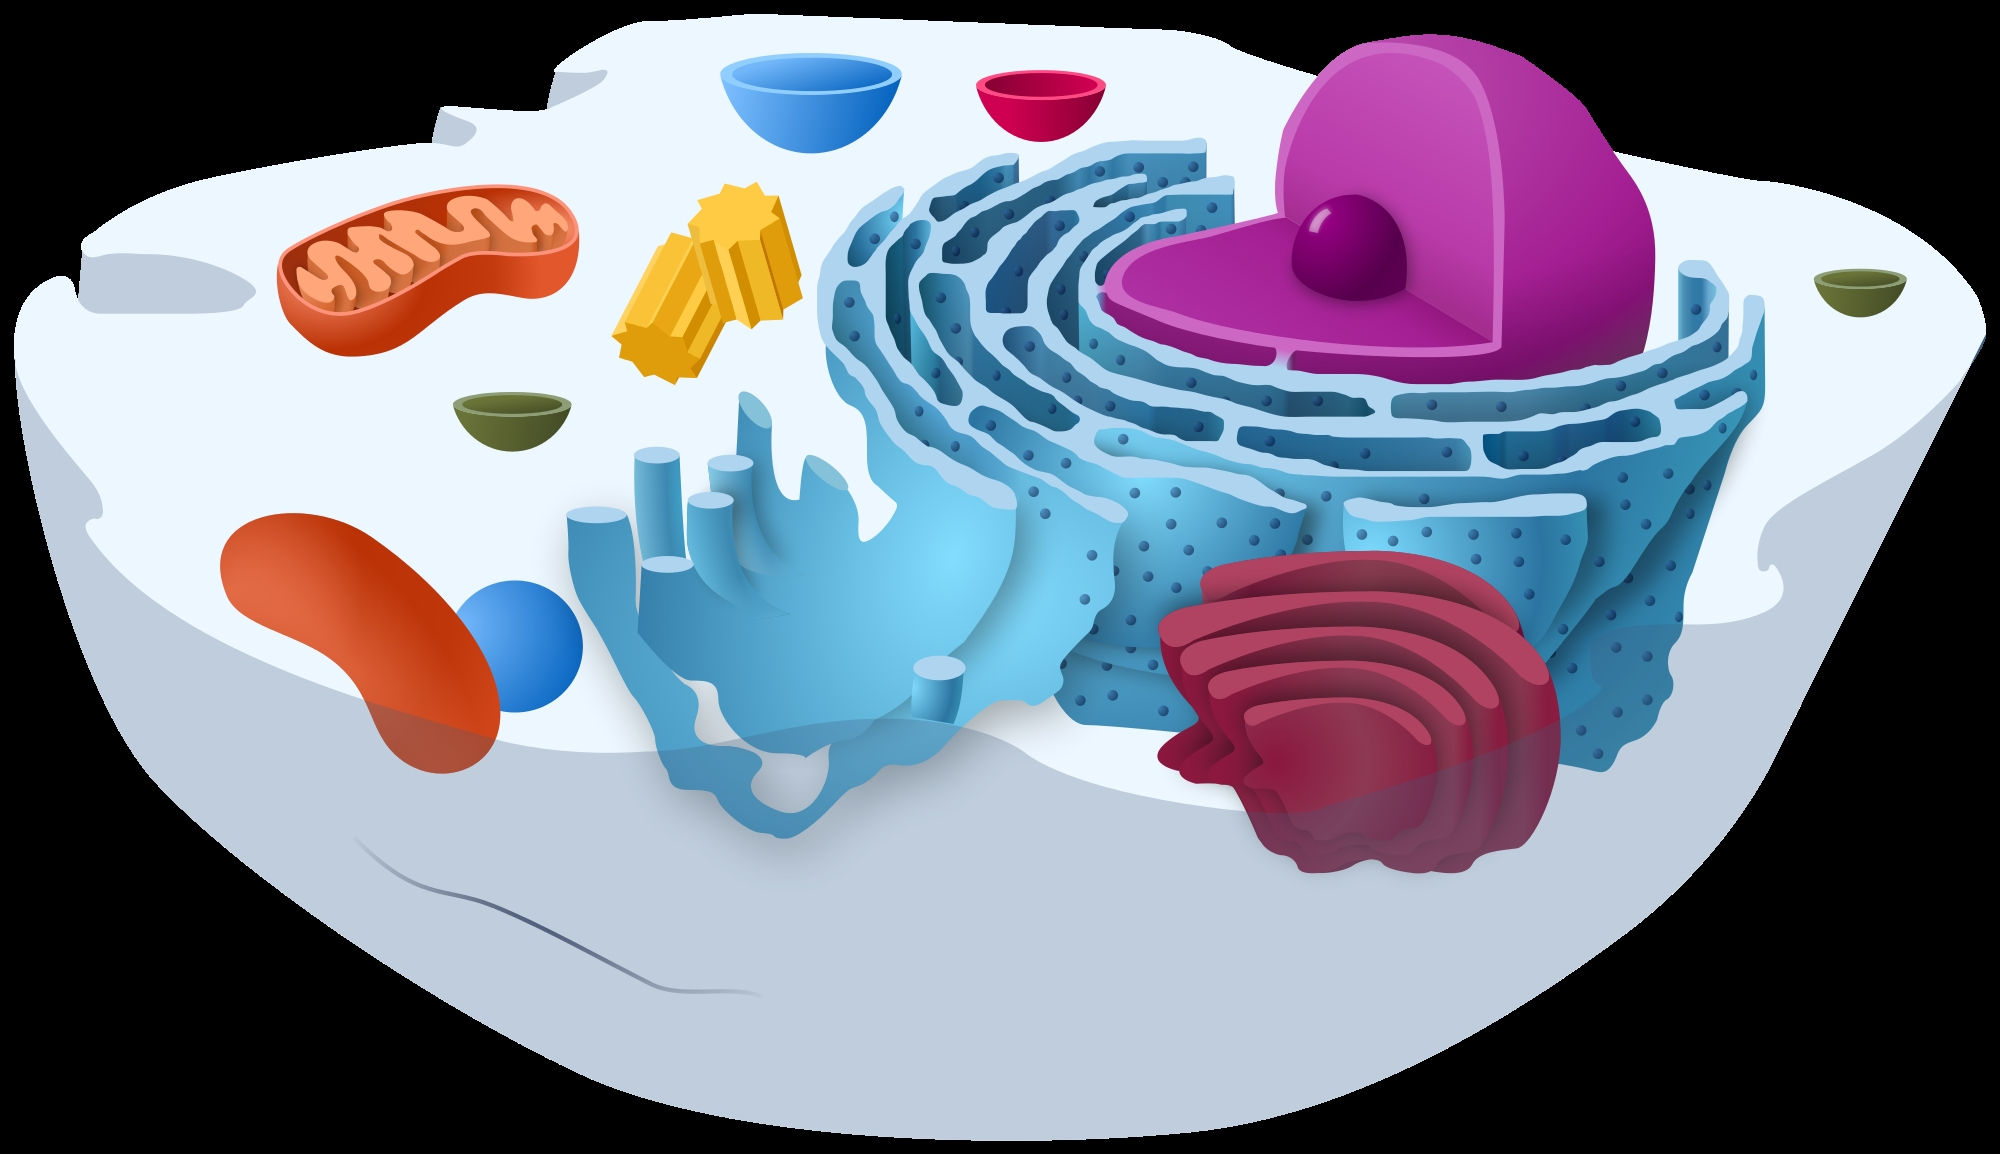
\includegraphics[width=0.9\textwidth]{Cell}
\end{figure}

\begin{figure}[H]
	\caption{Metabolism}\label{fig:metabolism}
	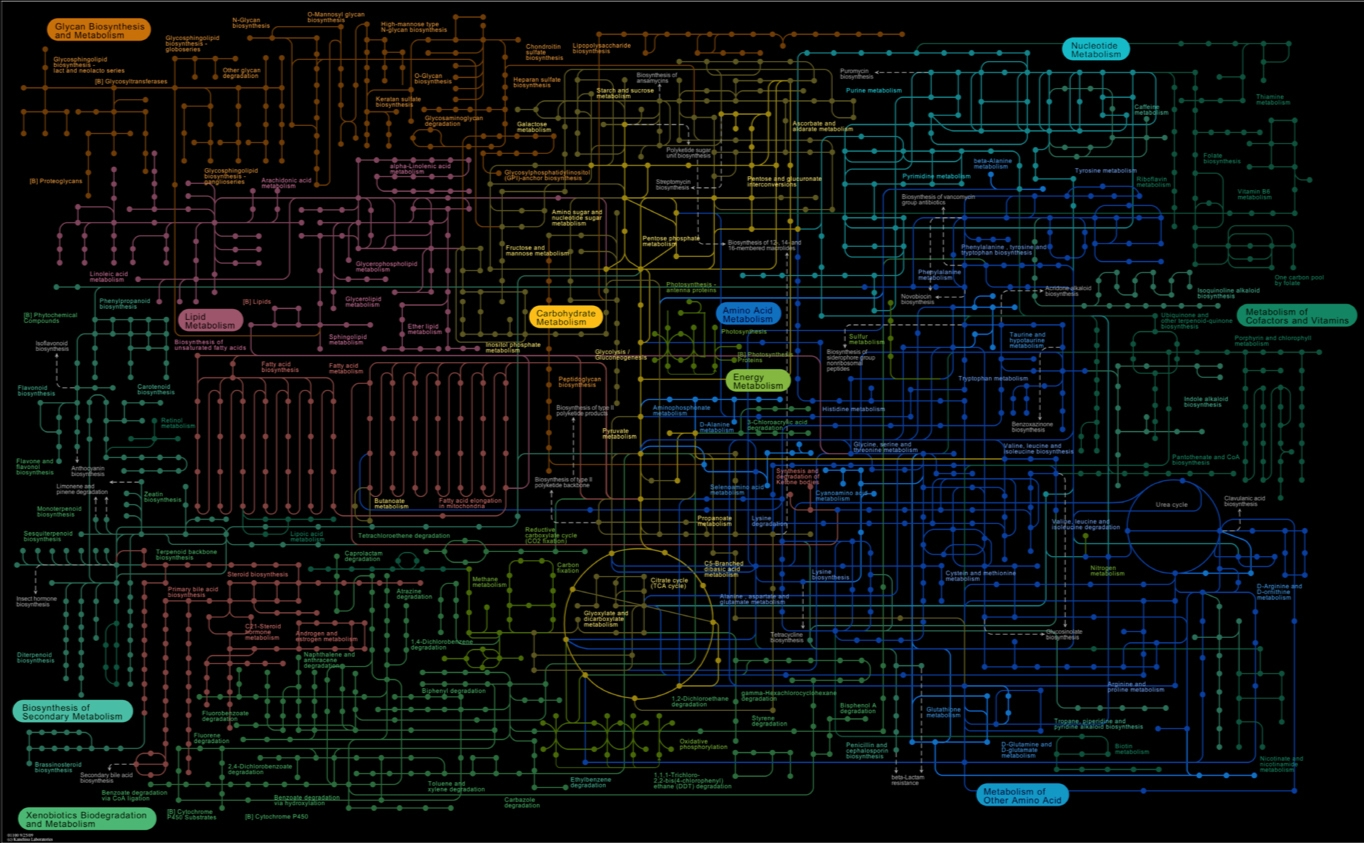
\includegraphics[width=0.9\textwidth]{Metabolism}
\end{figure}

\begin{figure}[H]
	\caption{Tardigrade--an extremophile that can live in space}\label{fig:tardigrade}
	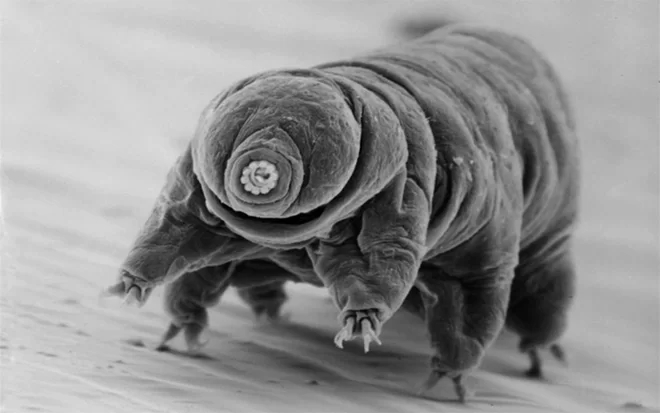
\includegraphics[width=0.9\textwidth]{Tardigrade}
\end{figure}


\begin{figure}[H]
	\caption{Two Headed Planaria}\label{fig:2headed:planaria}
	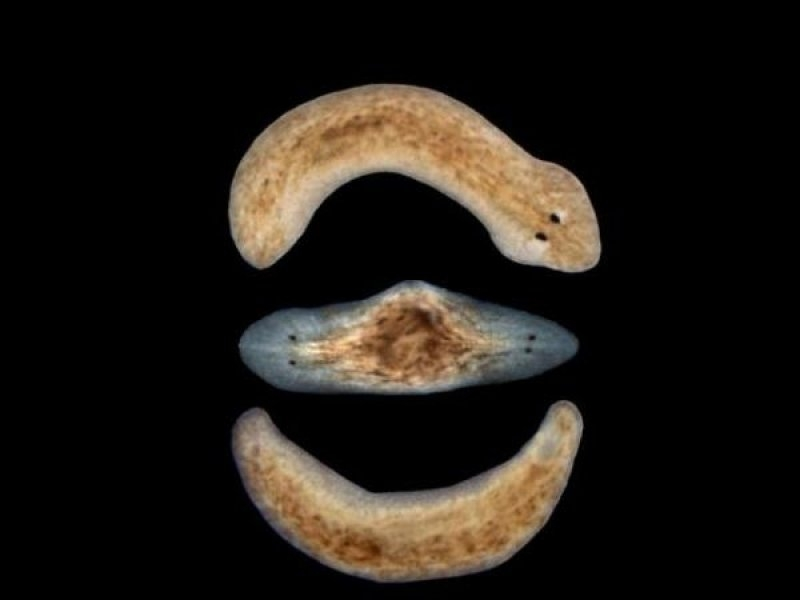
\includegraphics[width=0.9\textwidth]{TwoHeadedPlanaria}
\end{figure}

\begin{figure}[H]
	\caption{Social Insects: is the super-organism "alive"?}\label{fig:social:insects}
	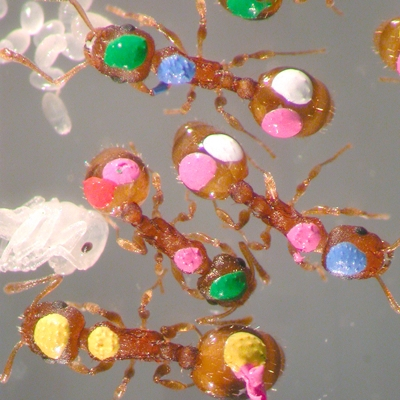
\includegraphics[width=0.9\textwidth]{SocialInsects}
\end{figure}

\begin{figure}[H]
	\caption{City}\label{fig:city}
	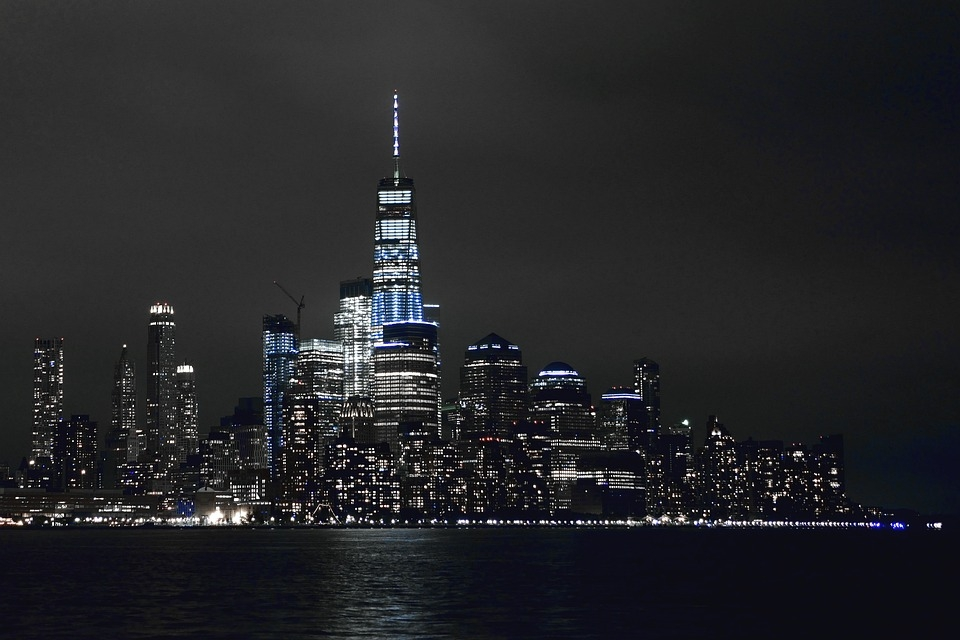
\includegraphics[width=0.9\textwidth]{City}
\end{figure}

\begin{figure}[H]
	\begin{subfigure}[b]{0.45\textwidth}
		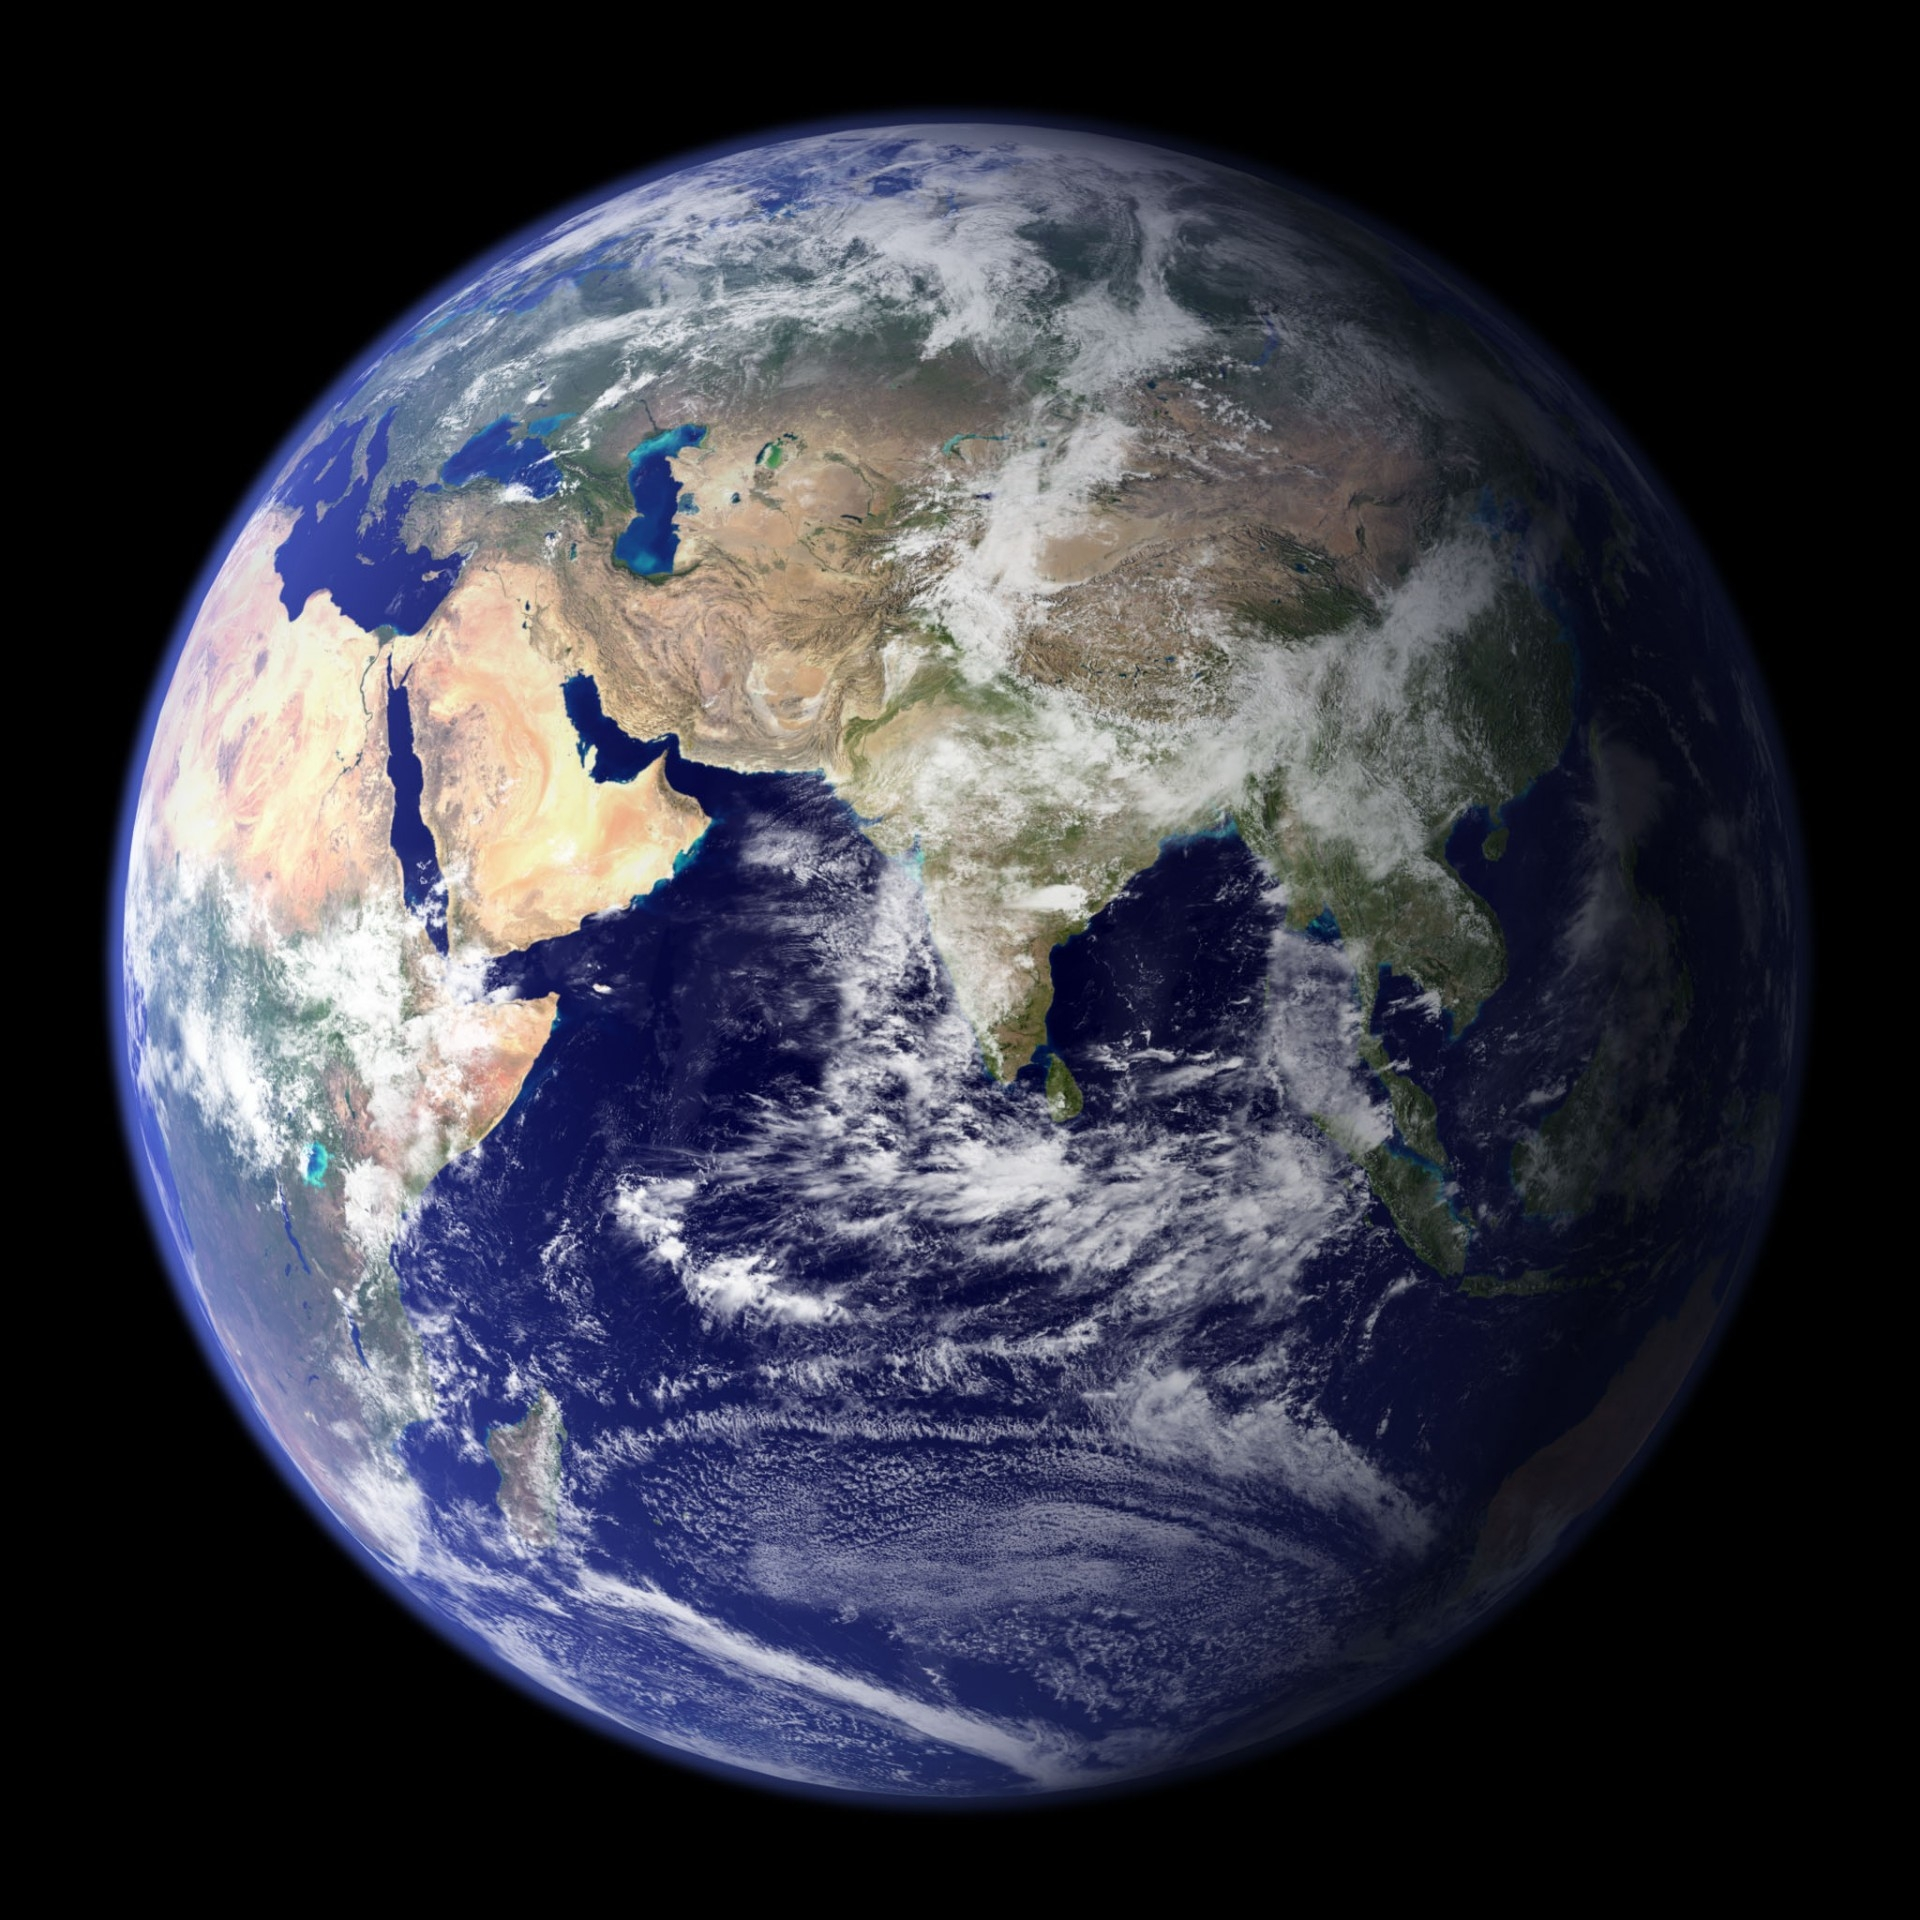
\includegraphics[width=\textwidth]{Globe1}
	\end{subfigure}
	\begin{subfigure}[b]{0.45\textwidth}
		\caption{Network representation of the global inventory of
			enzymatically catalyzed biochemical reactions}
		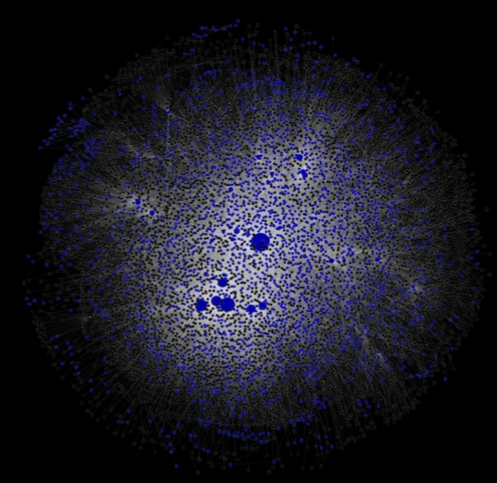
\includegraphics[width=\textwidth]{Globe2}
	\end{subfigure}
\end{figure}
\subsection{Weird Life}

\cite{hollants2011life}

\cite{kim2001life}

\cite[Chapter 6: Why Water? Toward More Exotic Habitats ]{board2007limits}

\cite{cejkova2014dynamics}

\section{Abstract and general Models for Life}

\cite{trifonov2011vocabulary}

\cite{cronin2016beyond}

\section{The Multiple Origins of Life}

\subsection{The Argument}

\subsection{Reversing the Arrow of Time}

\subsection{The Theory of the Adaptive Arrow of Time}

\cite{rockmore2018cultural}

\subsection{Evolutionary Agents}

\section{Evolutionary Computation}

\cite{mitchell1998introduction}
\cite{eiben2003introduction}
\cite{holland1992adaptation}
\cite{forrest1993genetic}
\cite{ma2014novo}
\cite{marshall2014evolution}


\section{Scaling}

\cite{anderson2013altered}
\cite{damuth1981population}
\cite{enquist1998allometric}
\cite{enquist2012land}
\cite{marquet2005scaling}
\cite{schmidt1984scaling}
\cite{tucker2014evolutionary}
\cite{west1997general}

\section{Energy}

\cite{odum1976energy}
\cite{odum1983systems}
\cite{schmidt1997animal}
\cite{brown2004toward}
\cite{sibly2012metabolic}
\cite{ernest2003thermodynamic}
\cite{savage2004predominance}
\cite{dell2011systematic}
\cite{kempes2017thermodynamic}

% end of text 

% glossary
\printglossaries

% bibliography go here
 
\bibliographystyle{unsrt}
\addcontentsline{toc}{section}{Bibliography}
\bibliography{origins,wikipedia}

\end{document}
